



\section{Analysis} \label{sec:analysis}

We now investigate how a variety of factors affect the default and counterfactual performance trends that we observed in \S\ref{sec:results}.
Unless otherwise specified, we only consider GPT-4 with 0-shot CoT, which has the strongest performance in our results above.

\subsection{``Commonness'' of Counterfactual Conditions} \label{sec:analysis-world-commonness}
Our counterfactual worlds are  not designed to be completely alien to the LMs but only less common than the assumed default case.
In this sense, the counterfactual-ness of these worlds is relative, and here we take a more nuanced look at how the commonness of these counterfactual conditions affects the default-counterfactual performance gap.
For example, in the arithmetic task, all models perform better in bases 8 and 16, likely due to their relative abundance compared to  bases 9 and 11.
In spatial reasoning, the smallest counterfactual performance degradation is usually from when the north and south directions are swapped---even exceeding the default task performance for PaLM-2---potentially because some programming libraries use an inverted $y$-axis, such as matplotlib (Python), ggplot (R), and D3 (JavaScript) (see \S\ref{sec:spatial-setup}).
For chord fingering, the common alternative drop-D tuning of guitars (DADGBE) leads to the highest counterfactual performance for GPT-4.
These correlations between the counterfactual performance and the commonness of the counterfactual worlds paint a more fine-grained picture than a binary default versus counterfactual distinction and point to a memorization-like
effect where the models perform better under more common conditions.

\begin{figure*}
     \centering
     \vspace{-2mm}
     \begin{subfigure}[b]{0.24\textwidth}
         \centering
        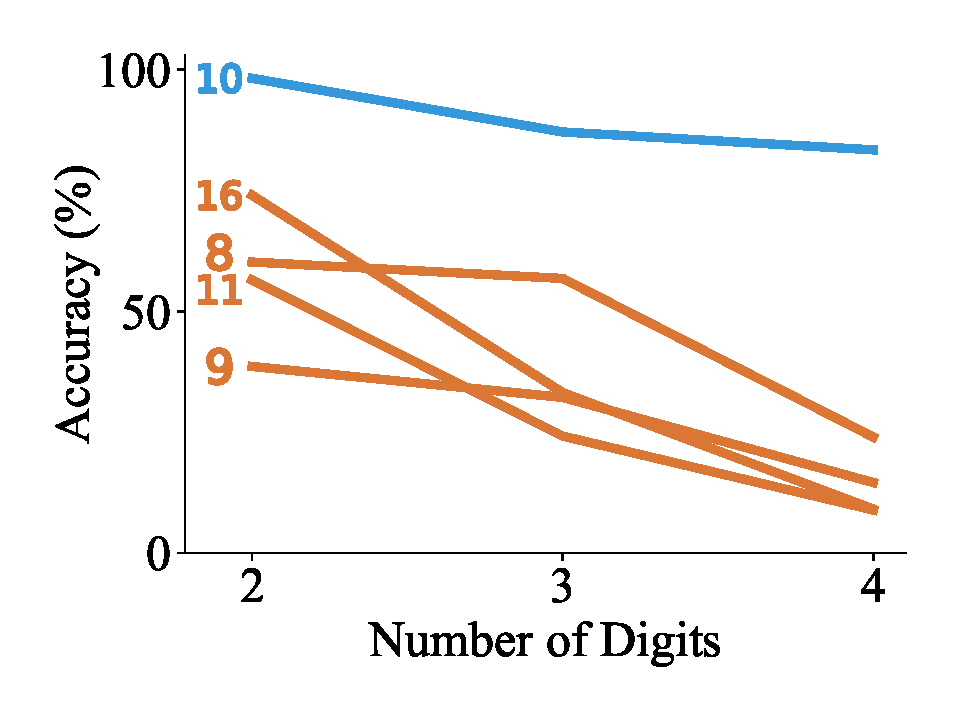
\includegraphics[width=\textwidth]{figures/math_ndigits.pdf}
        \caption{Addition accuracy with varying numbers of digits in the operands.}
        \label{fig:math-ndigits}
     \end{subfigure}
     \hfill
     \begin{subfigure}[b]{0.24\textwidth}
         \centering
        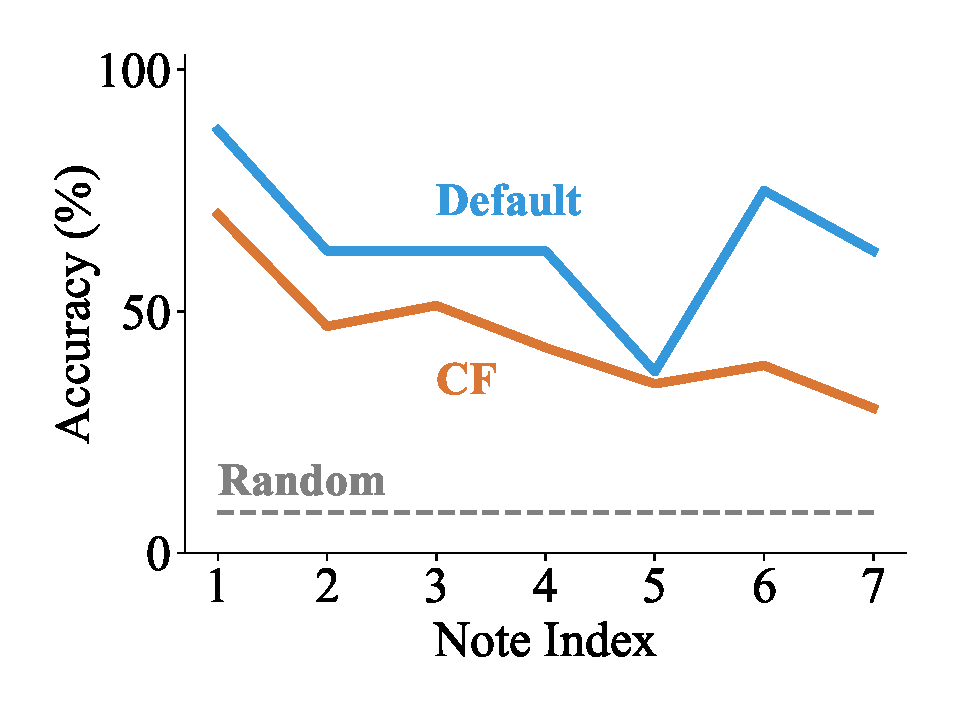
\includegraphics[width=\textwidth]{figures/note_index.pdf}
        \caption{Melody note recall accuracy broken down by the index of the note.}
        \label{fig:songs_by_n}
     \end{subfigure}
     \hfill
     \begin{subfigure}[b]{0.24\textwidth}
         \centering
        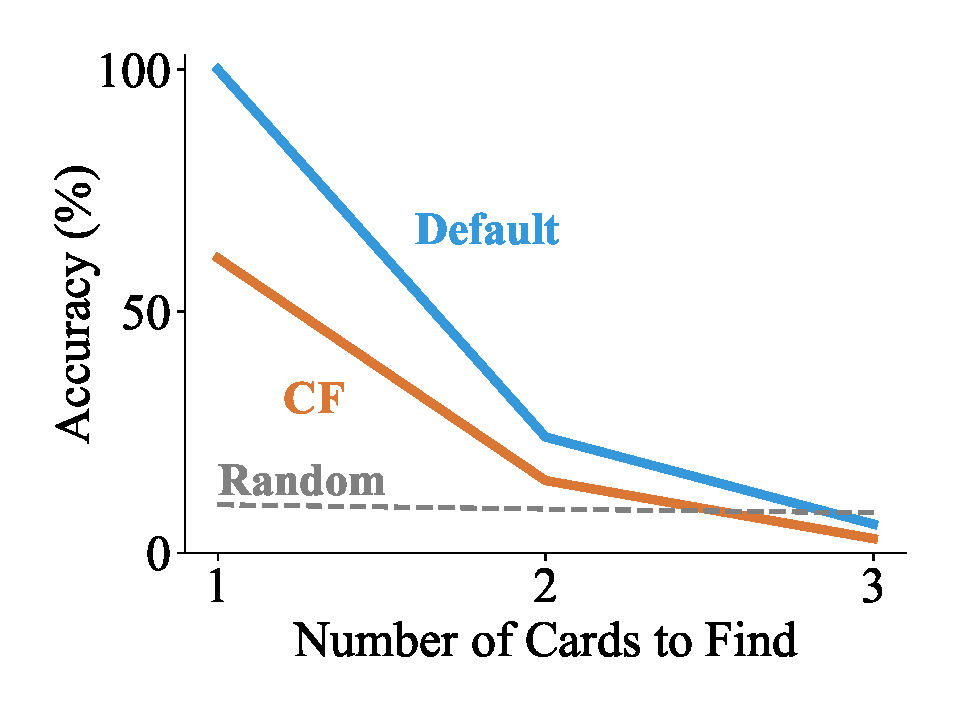
\includegraphics[width=\textwidth]{figures/set_nhints.pdf}
        \caption{SET identification accuracy when needing to find different numbers of cards in a SET.}
        \label{fig:set-nhints}
     \end{subfigure}
     \hfill
     \begin{subfigure}[b]{0.24\textwidth}
         \centering
        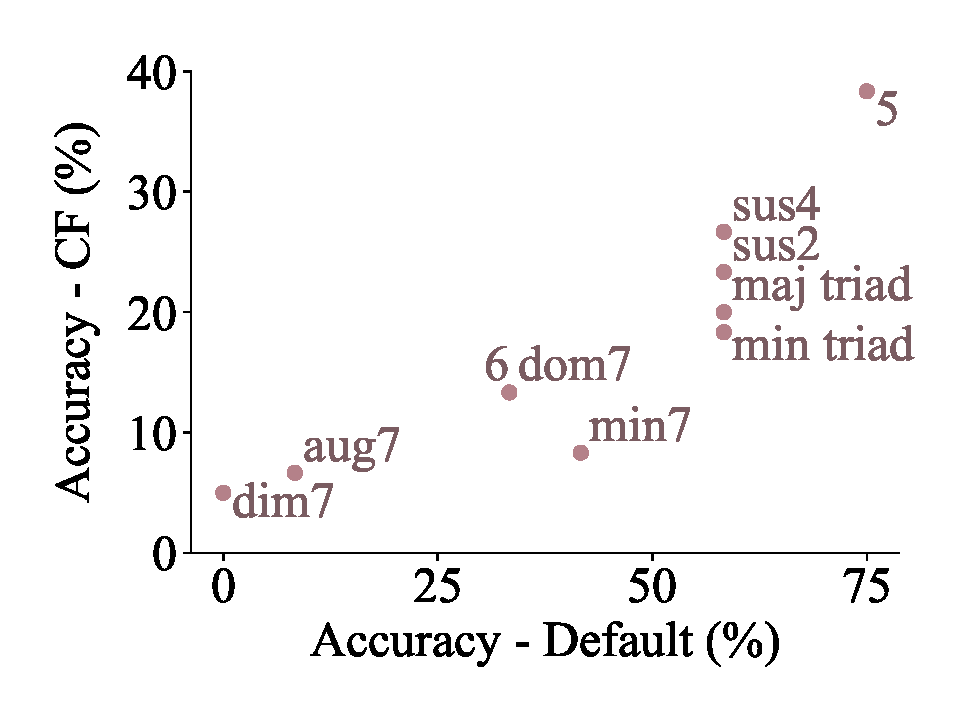
\includegraphics[width=\textwidth]
        {figures/chords_scatter.pdf}
        \caption{Fret placement accuracy by chord type. The $y$-axis averages over all altered tunings.}
        \label{fig:chords_by_type}
     \end{subfigure}
     
    \caption{Investigating the relationship between the default task performance and counterfactual performance, broken down by different factors. Only GPT-4 with 0-shot CoT results are shown. There is a consistent default-counterfactual correlation across task variants when varying different factors.}
    \vspace{-2mm}
    \label{fig:rc-relationship}
\end{figure*}

\begin{figure}[t!]
    \centering
    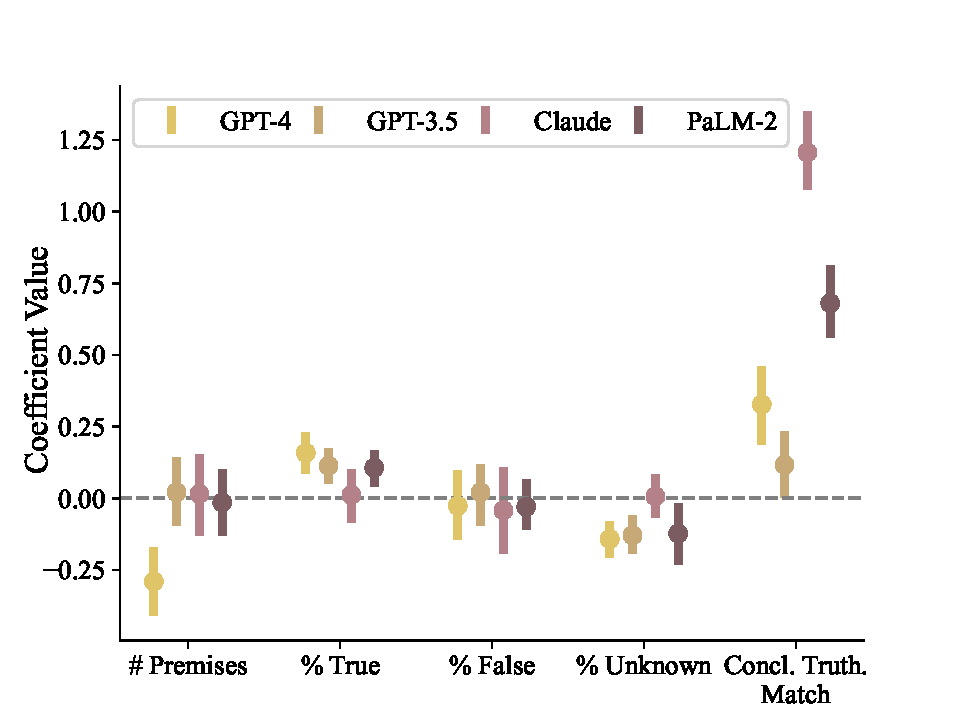
\includegraphics[width=0.48\textwidth]{figures/coefficients.pdf}
    \caption{Logistic regression coefficients of features that predict whether an LM correctly predicts the label of an instance. ``Concl. Truth. Match'' is a binary feature that is 1 iff the instance label matches the (LM-believed) truthfulness of the conclusion. The 95\% confidence intervals are also shown. LMs tend to predict more correctly when there are more true premises, when the instance label matches the conclusion truthfulness, but less correctly with more false and unknown premises.}
    \label{fig:folio-coefs}
    \vspace{-2mm}
\end{figure}

\subsection{Proximity between Default and Counterfactual Conditions} \label{sec:analysis-world-realness}

Another axis along which the counterfactual worlds differ is in their proximity to the default conditions.
For example, for the different arithmetic bases, bases 9 and 11 are \emph{closer} to base 10, but \emph{less common} than bases 8 and 16.
While the default-counterfactual gap is most affected by commonness for the arithmetic task,
for the guitar and ukulele tunings (other than the drop-D tuning), the LM performance  generally decreases monotonically with increasing distance from the original tunings.

The FOLIO dataset~\citep{han2022folio} enables another analysis of how proximity to the default conditions affects LM performance, \emph{without} counterfactual perturbations. This dataset was constructed to mostly follow common sense, with premises and conclusions deemed true in the real world. But this is not always the case, with premises like ``John can make meals which are popular at the party,'' whose factuality cannot be determined alone. 

We evaluate how the distance between the (LM-believed) real world and the world state described by the premises (occasionally counterfactual to the LM) influences the LM's performance by training a predictive model given features approximating this distance.
For each test instance, we ask the LMs whether the premises and conclusion are true, false, or uncertain. We train a logistic regression model to predict LM correctness on each test instance, using as features the total number of premises in an input, the proportion of the premises that are true/false/uncertain, as encoded by the LM, as well as whether the LM-predicted truthfulness of the conclusion matches the label of the instance. %

Figure~\ref{fig:folio-coefs} shows the learned coefficients of these features, as well as their 95\% confidence interval bootstrapping with 1,000 iterations~\citep{EfroTibs93}.
Ideally, a robust model should predict solely based on symbolic deduction and extralinguistic truthfulness information should not affect its accuracy. In other words, these features should all have coefficients 0 and have no predictive power with respect to the model's correctness. However, all LMs predict more correctly with more realistic (true) premises, and when the conclusion's LM-predicted truthfulness matches the label (indicating a tendency to predict the label solely based on the conclusion, ignoring premises). On the other hand, they perform worse when there are more false or uncertain premises.
Most of these trends are statistically significant. 
This means that the reasoning ability of LMs is affected by the distance between the (LM-believed) real world and the world state under which the LMs are expected to reason.

Overall, these results show that LMs tend to perform better on task variants that are closer to the default instantiation of a task.

\subsection{Relationship between Default vs. Counterfactual Performance} \label{sec:rc-relationship}

Recalling our formalization $h_{\text{LM}}(f, w, x)$ in \S\ref{sec:counterfactual-eval}, the previous two subsections analyzed how  the commonness of $w$ and its proximity to $w^\text{default}$ affect the observed patterns. We now explore how the counterfactual performance correlates with the default task performance by varying the other three elements: the task $f$, the input $x$, and the LM.

We first consider different task variants with various difficulties.
For arithmetic, beyond 2-digit addition, we also measure GPT-4's 3- and 4-digit addition performance (Figure~\ref{fig:math-ndigits}).\footnote{See \citet{dziri2023faith} for a related analysis but for multiplications.}
For note retrieval from melodies, we use the index of the inquired note as the proxy for  difficulty (Figure~\ref{fig:songs_by_n}).\footnote{This is not a new task variant as compared to the setup in \S\ref{sec:music-task}, but rather a decomposition of our original results.}
For SET, while our original task shows two cards and asks a model to find the missing one from a 3-card SET, we change the task to instead show one or none of the cards in a SET, while still requiring the model to identify the SET (Figure~\ref{fig:set-nhints}).
For all these task variants, we see a strong correlation between the original and counterfactual world performance.

We also see this effect when breaking down results by test instances $x$. In Figure~\ref{fig:chords_by_type}, we separate the chord types, and observe that the default task performance correlates with the counterfactual performance. Similarly, reexamining our main results in Figures~\ref{fig:results-1} and \ref{fig:results-2}, for most tasks, stronger models under default conditions are also stronger models under counterfactual conditions, and vice versa.
Overall, these correlations mean that the default task performance can be a good indicator of its counterfactual performance, and hence we should not discount the utility of traditional evaluations.\footnote{Though these correlations are not necessarily causal.}

Furthermore, despite our evidence of LMs' overfitting to the default task conditions, 
these correlations also signify some degree of reasoning that is transferable between the default and counterfactual worlds.
This highlights that the question in our title, ``Reasoning or Reciting?'', is not a dichotomy, but rather they can co-exist in a continuum.
For example, revisiting the arithmetic results with more digits (Figure~\ref{fig:math-ndigits}), in addition to the default-counterfactual correlation, we also see an effect of memorization:
the base-10 performance decreases much more slowly than the other bases. When the input-output mappings are memorized, increased complexity would not affect the default task accuracy much; but when the counterfactual instances are not memorized, the task complexity should inversely correlate with model performance.


Occasionally, this default-counterfactual correlation trend is reversed.
In the spatial reasoning task, for example, GPT-4 achieves the best accuracy under default conditions with 0-shot CoT, but it also suffers from the largest counterfactual performance degradation. PaLM-2 performs worse under default conditions, but is the most robust to counterfactual perturbations.
An obvious possible explanation is that these models could be trained on different data, and are hence familiar with different conditions. Nevertheless, \citet{mckenzie2023inverse}, who found a similar trend but with respect to pretraining FLOPs and termed it ``inverse scaling,'' also provided a memorization-based explanation: they observed that when a task contradicts with pretraining texts, similar to how our counterfactual conditions deviate from the default conditions in pretraining, larger LMs tend to rely on the pretraining text and, in turn, fail at the contradictory task.



\subsection{0-Shot Chain-of-Thought Prompting}

Consistent with prior findings~\citepia{chen2022program,dasgupta2022language}, we generally observe 0-shot CoT to be helpful for most cases.
There are, however, exceptions. For example, 0-shot CoT substantially hurts PaLM-2's addition performance in base-10 and 16, and consistently degrades GPT-4 and GPT-3.5's chord-playing performance for the default tuning. This may be due to a model pragmatically inferring that a task is more difficult than it actually is when  explicitly asked to ``\texttt{think step by step}'', and this ``overthinking'' on simple tasks could lead to mistakes~\citep{kojima2023large}. It is also possible that these are due to memorization: the model could have memorized the specific input-output mapping of a task, without understanding how to derive the output from the input, and when explicitly instructed to spell out that process, it makes more errors~\citep{zhang2023language}. 


\begin{figure}[t!]
    \centering
    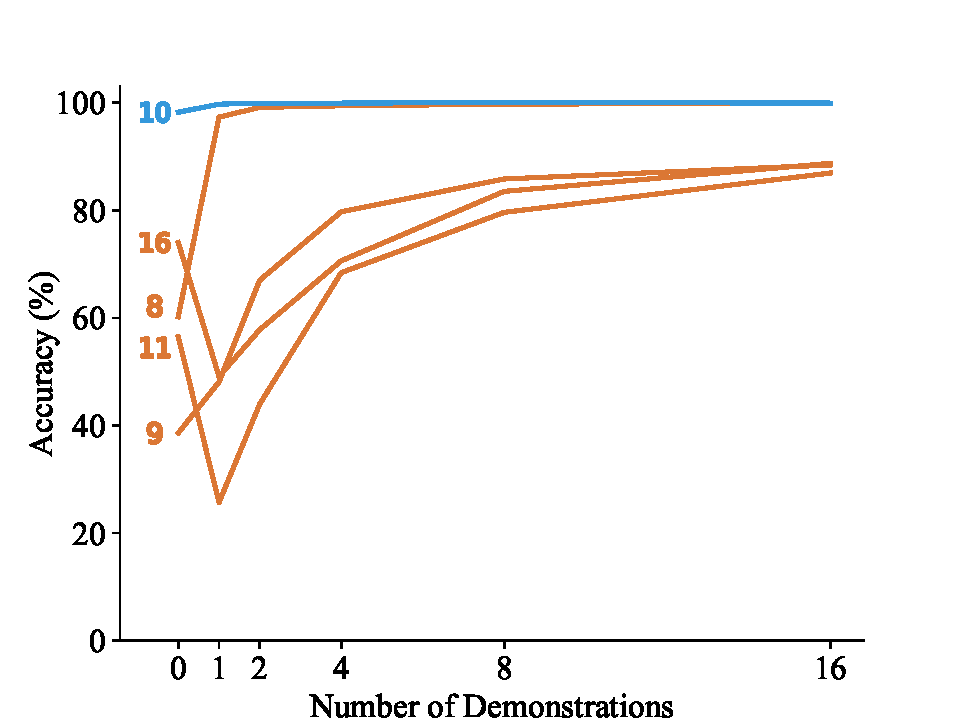
\includegraphics[width=0.45\textwidth]{figures/math_icl.pdf}
    \caption{Two-digit addition accuracy when given different numbers of demonstration examples. The default-counterfactual gap reduces, but is not eliminated.}
    \vspace{-4mm}
    \label{fig:math-icl}
\end{figure}

\subsection{Few-shot Demonstrations} \label{sec:analysis-icl}
We study if additional demonstration examples using in-context learning~\citep{gpt3} bridges the default-counterfactual gap. For the arithmetic task, we construct few-shot CoT prompts~\citep{nye2021work,wei2022chain} and prepend up to 16 samples. As shown in Figure~\ref{fig:math-icl}, while the gap is reduced, it is still substantial for bases 9, 11, and 16. Moreover, the accuracy improvement with more demonstrations plateaus towards 16-shot, suggesting that the default-counterfactual gap  is unlikely to  be eliminated by simply adding more demonstrations (at least for arithmetic).\footnote{An interesting pattern is that bases 11 and 16 \emph{suffer} from 1-shot demonstration than 0-shot. We hypothesize that this may be due to these being the two bases with letter digits.}

\subsection{Qualitative Analysis of Drawing Results}

We conduct a qualitative error analysis on the drawing task and show some examples in Figure~\ref{fig:drawing_vis}.  We first note that GPT-4 successfully passes the CCC for these cases (see \S\ref{sec:drawing-task}; but not displayed here), indicating that it understands the flip/rotation instructions.  However, the objects in the counterfactual worlds are often not flipped or rotated. Even when they are transformed appropriately, the resulting drawing is often simplified or of worse quality (e.g., \texttt{Unicorn}, \texttt{Cake}). We also observed much more syntactically invalid programs in the counterfactual cases for GPT-3.5.\footnote{On average, the number of parseable programs generated by GPT-3.5 drops from 99\% in the default condition to 62\%, 71\%, and 75\% for the vertically flipped, 90\textdegree\ rotated, and 180\textdegree\ rotated settings, respectively.} These results indicate that even when a model can perform a task in the counterfactual setup, its capabilities are reduced.



\begin{figure}[t!]
    \centering
    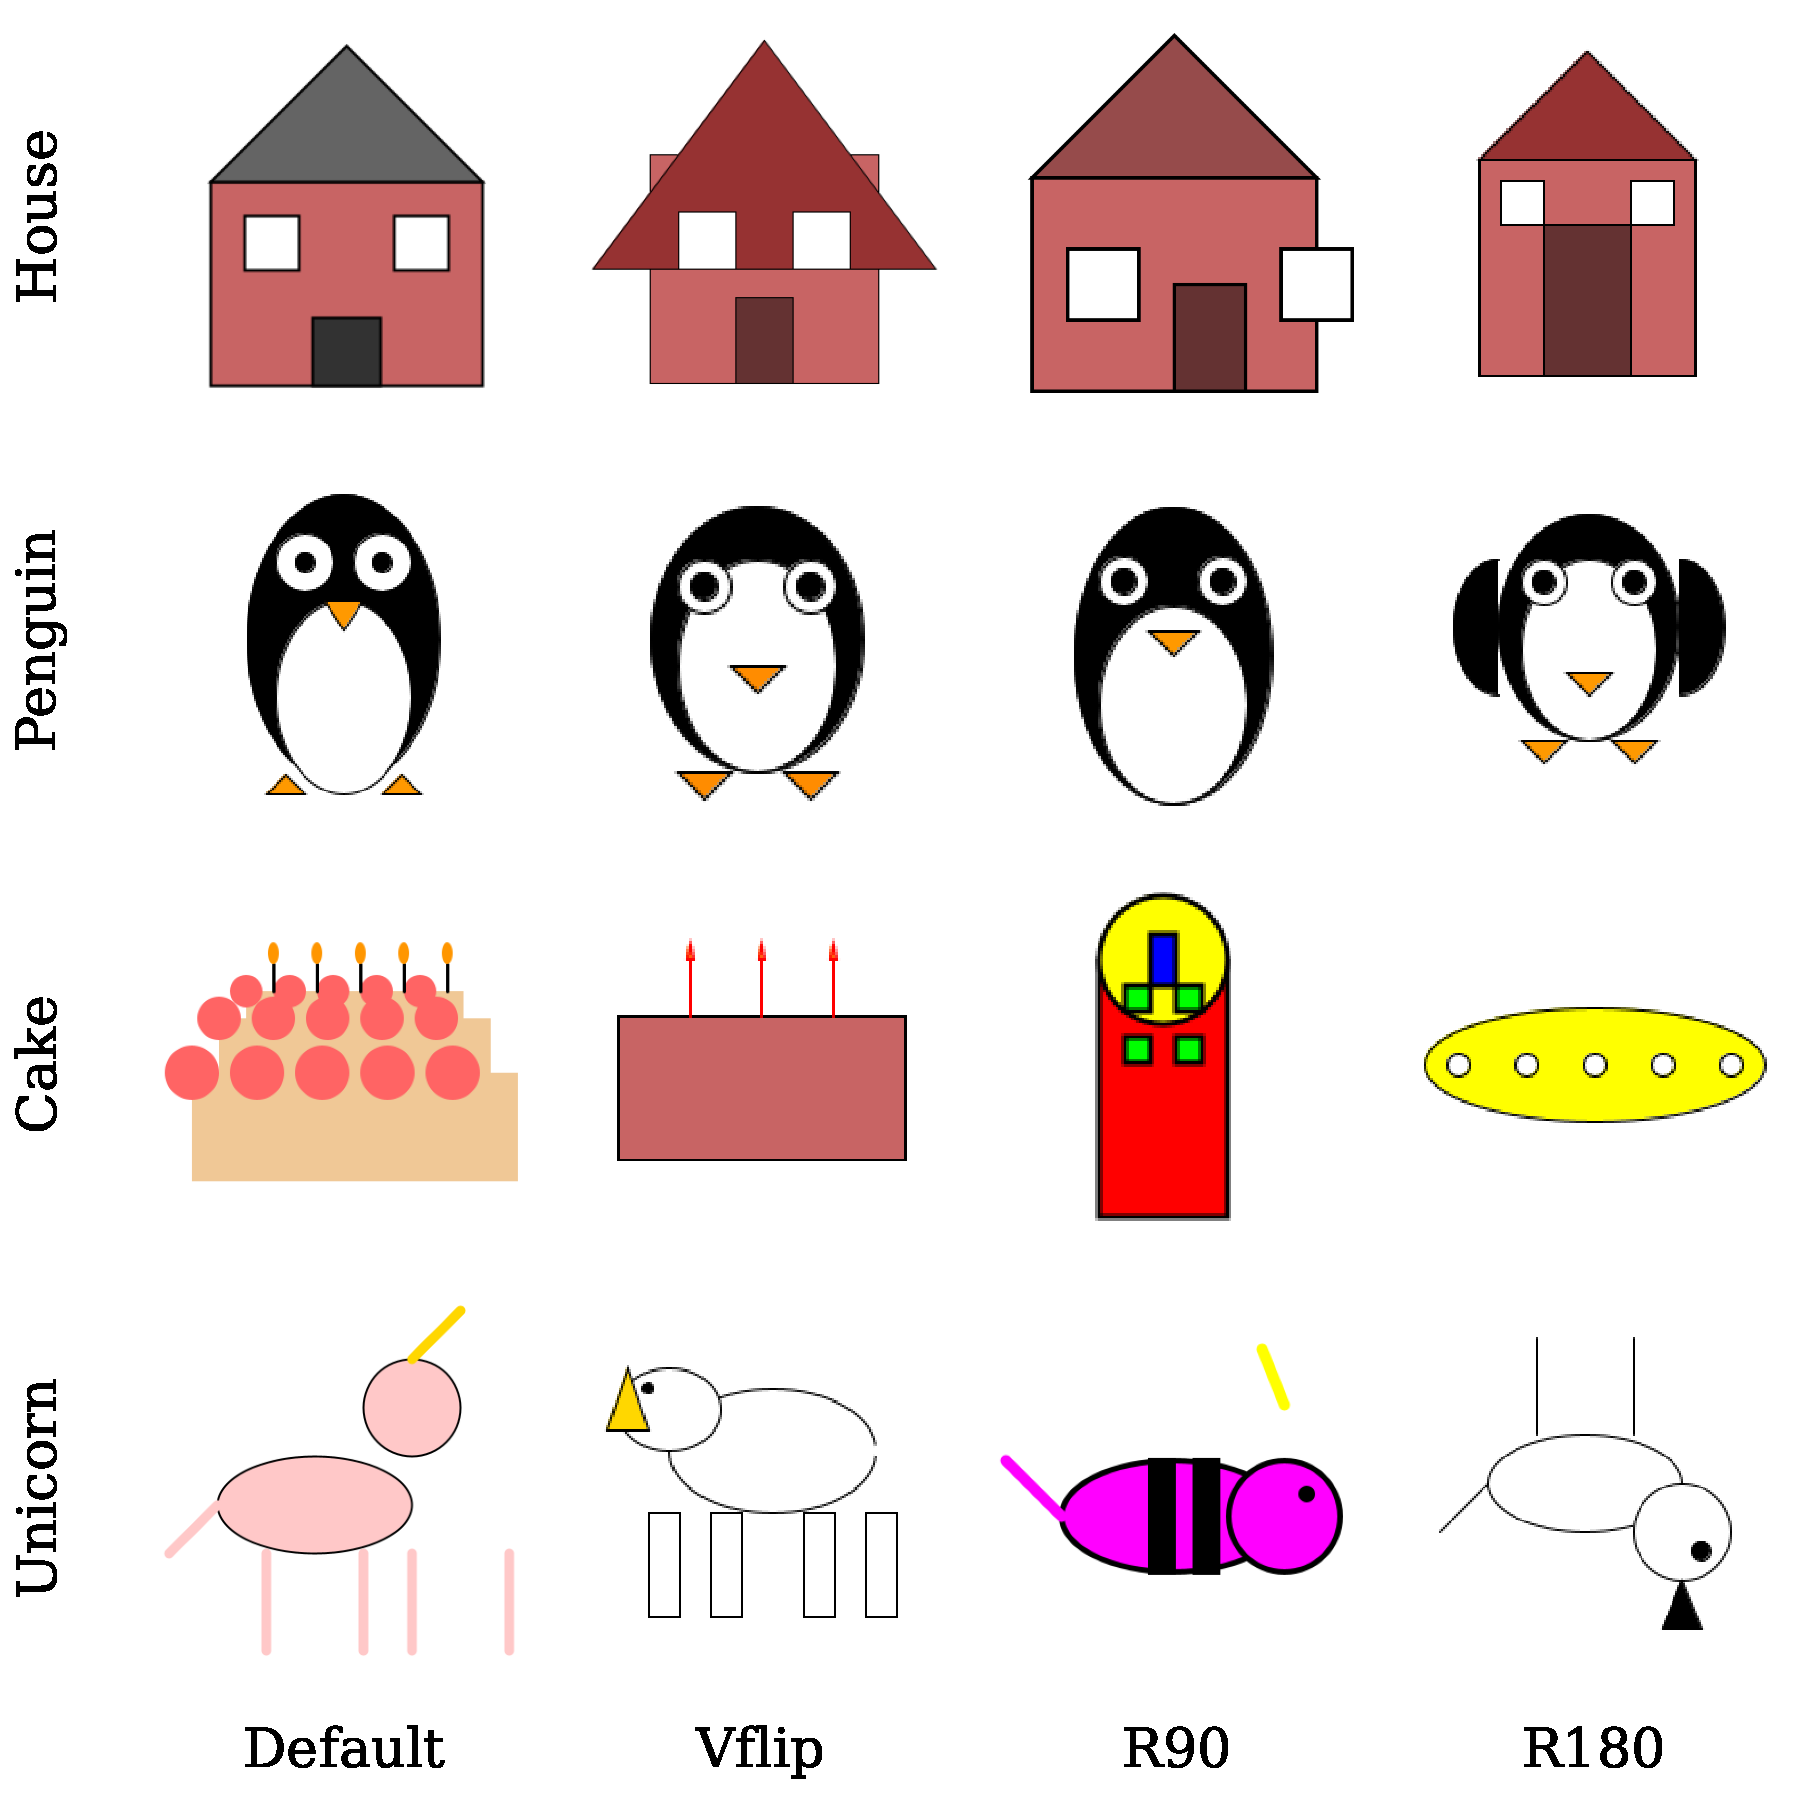
\includegraphics[width=0.48\textwidth]{figures/drawing_vis.pdf}
    \caption{Visualizations of objects drawn by GPT-4 under the default (upright) and counterfactual conditions: vertical flip (Vflip, i.e. upside-down), rotates 90 degrees (R90), and 180 degrees (R180). In all cases, the CCC (not shown) passes.
    We show the original output, without flipping/rotating back as in our quantitative evaluation (\S\ref{sec:drawing-setup}).
    For the counterfactual settings, GPT-4 either does not transform the objects as instructed (e.g., house and penguin) or struggles to draw meaningful objects (e.g., cake and unicorn).}
    \vspace{-2mm}
    \label{fig:drawing_vis} 
\end{figure}
